\documentclass[12pt]{article}

\usepackage[english]{babel}
\usepackage[utf8]{inputenc}
\usepackage{mathtools}
\usepackage{graphicx}
\usepackage[colorinlistoftodos]{todonotes}
\usepackage[margin=0.9in]{geometry}
\usepackage{multicol}

\usepackage{csquotes}
\usepackage[style=verbose-ibid,backend=biber]{biblatex}
\bibliography{sample}

\title{How to use axions to shine light through walls}

\author{Nicholas Montague}

\date{\today}

\begin{document}
\maketitle

\begin{abstract}
The axion is a hypothetical particle, introduced by the Peccei-Quinn theory in 1977 as a solution to the strong CP problem in quantum chromodynamics. The axion, if it exists, must have a very small mass, and must be very weakly interacting with baryonic matter, giving it the abbreviation WISP (Weakly Interacting Sub-ev Particle). The predicted attributes of the axion would give it the ability to pass directly through an opaque wall without obstruction, and this is how the ALPS experiment (Any Light Particle Search) at DESY in Hamburg is exploring the possibility of their existence. In this report, we will use matrix methods to reproduce the relationship between axion mass and axion coupling as published by the ALPS experiment \autocite{Ehret, K. et al (2010). New ALPS results on hidden-sector lightweights} in 2010, using their conversion probability to plot the result. Note that all equations, unless otherwise stated, are in natural units ($c=1$, $\hbar = 1$).
\end{abstract}

\section{Introduction}

In particle physics, there is a lot of speculation over why quantum chromodynamics (QCD) does not seem to break CP-symmetry in the strong interaction \autocite{Peccei, R.D. (2006). The Strong CP Problem and Axions} when it should. CP-symmetry is the idea that if we take a system, perform charge conjugation so that all particles become their antiparticles, and also 'flip' the system so that all lefts become rights and vice-versa, the laws of physics remain unchanged. A way to overcome this problem, is to promote the CP violating parameter to a new field, called the axion field, and introduce its propagating particle, the axion. By introducing this new particle, the QCD Lagrangian is altered slightly, as this accounts for the error in the CP-symmetry. 
The axion is also of great interest to the standard model, as if its mass lies in a certain low range, it is a possible component for cold dark matter \autocite{Duffy, L.D., Bibber, K. (2009). Axions as Dark Matter Particles}  that has been observed, but not identified. The two criteria that must be satisfied to be a possible dark matter candidate are: (1) a very cold population of axions could be present in our universe in large enough quantities to provide the required dark matter energy density and (2) they are effectively collisionless. There have been several experiments that have attempted to detect the presence of axions, using a range of predicted properties of axions. 
One these was the Polarizzazione del Vuoto con LASer (PVLAS) in Italy, with ideas put forward by Luciano Maiani, Roberto Petronzio and Emilio Zavattini in 1986 \autocite{Maiani, L., Petronzio, R., Zavattini, E.(1986). Effects of nearly massless, spin-zero particles on light propagation in a magnetic field}. PVLAS searches for a slight rotation in the polarisation plane of light shining through a strong electromagnetic field. One interpretation \autocite{Ringwald, D. (2006). Axion interpretation of the PVLAS data?} of this effect includes the production of a small particle (an axion) with a mass $m_a~meV$ which couples to a pair of photons.
Another experiment is the Axion Dark Matter Experiment\autocite{Duffy, L.D. et al. (2006). A High Resolution Search for Dark-Matter Axions} (ADMX) at the University of Washington, which searches for axions in the local galactic dark matter halo using a microwave cavity detector. Although no axion signal was found, they were able to place a limit on the mass of the axion, between $1.98-2.17 \mu eV$. 
The particular experiment that we will be concentrating on, is the "Light Shining Through Walls" experiment (LSW), in particular, results published by the ALPS Collaboration at the Deutsches Elektronen-Synchrotron in Hamburg, in the paper 'New ALPS results on hidden-sector lightweights' \autocite{Ehret, K. et al (2010). New ALPS results on hidden-sector lightweights}. They were able to place limits on the probability of photon-axion-photon conversions to a very high precision $(10^{-25})$. 


\section{Theory}
\label{sec:theory}

A LSW experiment takes advantage of the fact that axions are very weakly interacting to detect their presence. The experimental setup of the ALPS collaboration consists of a $4.4m$ long vacuum chamber heading directly into a wall, and the equivalent on the other side of the wall (see 1) \autocite{http://inspirehep.net/record/791128/plots, 07/05/2014}. A strong magnetic field is applied perpendicular to the vacuum tubes, and a laser emits a beam of photons through the magnetic field. At a photon-photon vertex, when two photons interact with each other, they can couple, which leads to the production of an axion. As the axion is very weakly interacting, it can pass directly through the opaque wall, whereas all the photons are absorbed or reflected by it. On the other side of the wall, the axion can decay into two photons, in a reverse way to how it was created. If the detector on the right picks up any photons, this means that light has seemed to have travelled through the wall, but infact it is another, weakly interacting particle that has surpassed the wall, most probably an axion.

\begin{figure}[h]=
\centering
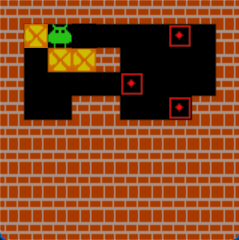
\includegraphics[width=0.7\textwidth]{Images/sokoban_cas_1.png}
\caption{\label{fig:RMPfig23.jpg}This diagram shows a simple layout for the LSW experiment. Taken from inspirehep.net}
\end{figure}

For the ALPS experiment, a $5T$ magnetic field was used, provided by a HERA superconducting dipole magnet, and the photons were produced by a $532nm$ laser. In order to increase the power of the laser (to improve the conversion probability), the laser was shone through a potassium titanyl phosphate (PPKTP) crystal. However this high intensity of the fundamental frequencies also caused second and higher order modes to increase in intensity. By reducing the waist size of the system, the second order harmonic beam can be reduced by a factor of 100, whereas the first order harmonic is only reduced by a factor of 15. They were limited to using a laser power of $5W$, as when this was increased to $8W$, an effect called gray-tracking was detected in the setup.
After several 10 hours of the laser running, the power build-up started to degrade. This was found to be due to a slight degradation in the quality of mirrors used to direct the laser beam. 
Obviously a perfect vacuum is not achievable in a laboratory. The two vacuum chambers were filled with $99.9995\%$ pure argon, which has a refractive index close to one. The relative change of the refractive index in the chambers was estimated to produce a negligable error.
It was important that the structure of the system was very stable and rigid, especially on the light tight box with the detector and camera in, as these had to be removed to access the wall in the centre. The camera had to be posioned very precisely each time it was removed, and this error was determined to be less than $6\mu m$. 
Future improvements to the ALPS experiment include increasing the length of the vacuum chambers, directly increasing the probability that a conversion will occur in the increased distance, and also increasing the magnetic field strength across the vacuum chambers. 2017 hopes to see the completion of ALPS-IIc \autocite{https://alps.desy.de/e141064, 11/05/2014}, with a 100 metre long cavity on either side of the wall, and magnets covering this entire distance.



\section{Method}
\label{sec:method}

Start with a stationary wave equation for particles propagating along the z axis of a system, 

\begin{equation}
\left(\omega^2+\partial_z^2+\left( \begin{array}{ccc}
Q_{perp} & 0 & 0 \\
0 & Q_{para} & {\frac{B\omega}{M}} \\
0 & {\frac{B\omega}{M}} & -m_a^2 \end{array} \right)\ \right)\
\left( \begin{array}{c} 
A_{perp} \\ 
A_{para} \\
a \end{array} \right) = 0 
\end{equation}


where $\omega$ is the frequency of light, $Q_{j} = 2\omega^2(n_j-1)$, $n_j$ is the refractive index in the $j$ direction, $B$ is the transverse part of the magnetic field strength, $M$ is inversely proportional to the coupling strength and $m_a$ is the axion mass. $A_{perp}, A_{para}$ and $a$ are the perpendicular and parallel amplitudes of the photon states and the amplitude of the axion state respectively. This differential equation will prove difficult to solve, as there are three coupled equations in three different dimensions.

\subsection{Simplification to Two Dimensions}

A simplification can be made for the term $(\omega^2 + \partial_z^2)$ by factorising into $(\omega+i\partial_z)(\omega-i\partial_z)$, and noticing that, in natural units, $i\partial_z = k$. At this point, an approximation may be introduced, by assuming that the refractive index is equal to that of a vacuum, so $n\approx 1$, and $k=n\omega$ resulting in $k\approx\omega$.
Applying this approximation and dividing through by $2\omega$, \textbf{(1)} may be rewritten, 

\begin{equation}
\left(\omega+\left( \begin{array}{ccc}
\Delta_{perp} & 0 & 0 \\
0 & \Delta_{para} & \Delta_M \\
0 & \Delta_M & \Delta_a \end{array} \right)-i\partial_z\right)\
\left( \begin{array}{c} 
A_{perp} \\ 
A_{para} \\
a \end{array} \right) = 0 
\end{equation}

where all $\Delta's$ are the previous matrix elements reduced by $2\omega$.
As the only interest is in the parallel photon (going towards the wall) and the axion field, $A_{perp}$ and the $\Delta_{perp}$ row and column can be neglected, and the system can be described by the $2x2$ matrix equation, 

\begin{equation}
\left(\omega+\left( \begin{array}{ccc}
\Delta_{para} & \Delta_M \\
\Delta_M & \Delta_a \end{array} \right)
-i\partial_z \right)
\left( \begin{array}{ccc} 
A_{para} \\
a \end{array} \right) = 0
\end{equation}

As this is a two dimensional matrix equation, all terms must be matrices, and the non-matrix variables may be written as products of the identity matrix, so they become

\begin{equation*}
\left( \begin{array}{ccc}
\omega & 0 \\
0 & \omega \end{array} \right) and 
\left( \begin{array}{ccc}
i\partial_z & 0 \\
\ 0 & i\partial_z \end{array} \right)
\end{equation*}

Notice that the approximation of $n\approx 1$ means that $Q_j = 2\omega^2(n_j-1)\approx 0$, so $\Delta_{para}$ can be neglected, and some simple rearranging yields the two dimensional differential matrix equation

\begin{equation}
i\partial_z \left( \begin{array}{ccc}
A_{para} \\
a \end{array} \right) = \left( \begin{array}{ccc}
\omega & \frac{B}{2M} \\
\frac{B}{2M} & \omega-\frac{m_a^2}{2\omega} \end{array} \right)
\left( \begin{array}{ccc}
A_{para} \\
a \end{array} \right)
\end{equation}

This gives two coupled differential equations, which are still not simple and straightforward to solve, as they are still coupled to each other. 

\subsection{Diagonalisation of the Matrix}

A matrix can be written as a product of its eigenvectors and its diagonalised matrix, in the form $\textbf{A} = \textbf{PDP}^{-1}$, where $\textbf{P}$ and $\textbf{P}^{-1}$ are eigenvectors of $\textbf{A}$, 

\begin{equation*}
\textbf{D} = \left( \begin{array}{ccc}
d_1 & 0 \\
0 & d_2 \end{array} \right)
\end{equation*}

and, in this case, $\textbf{A}$ is the 2x2 matrix from equation $(4)$, 
\\
\begin{equation*}
\textbf{A} = \left( \begin{array}{ccc} \omega & \frac{B}{2M} \\ \frac{B}{2M} & 
\omega-\frac{m_a^2}{2\omega} \end{array} \right)
\end{equation*}
\\
With a matrix in its diagonalised form, there are no longer any cross-terms in the matrix multiplication, meaning that, for equation $(4)$, the differential equations will no longer be coupled to each other, and will become much easier to solve. By diagonalising the 2x2 matrix, equation $(4)$ will be able to be rewritten in the form

\begin{equation}
i\frac{\partial}{\partial_z} \left( \begin{array}{ccc} x_1 \\ x_2 \end{array} \right) = \left( \begin{array}{ccc} d_1 & 0 \\ 0 & d_2 \end{array} \right) \left( \begin{array}{ccc} x_1 \\ x_2 \end{array} \right)
\end{equation}

where $d_1$ and $d_2$ are the eigenvalues, and $x_1$ and $x_2$ are the components of the matrix $\textbf{X}$ defined by $\textbf{X} = \textbf{P}^{-1} \left( \begin{array}{ccc} A_{perp} \\ a \end{array} \right)$.

\subsection{Finding the Eigenvalues}

To find the eigenvalues of the matrix, use the equation 

\begin{equation}
\left| \begin{array}{ccc}
\omega - \lambda & \frac{B}{2M} \\
\frac{B}{2M} & \omega - \frac{m_a^2}{2\omega} - \lambda \end{array} \right| = 0
\end{equation}

Solving this for $\lambda$, and using the quadratic equation, yields the unsightly result 

\begin{equation}
\lambda = \frac{2\omega - \frac{m_a^2}{2\omega}\pm \sqrt{1+\frac{4B^2\omega^2}{M^2m_a^4}}}{2}
\end{equation}

However, we can define $tan2\theta = \frac{2B\omega}{Mm_a^2}$ and using the substitution $1+tan^2\theta = sec^2\theta$, reduces equation$(7)$ to 

\begin{equation}
\lambda = \omega \pm \frac{m_a^2}{4\omega} (sec2\theta \mp 1)
\end{equation}

Next, notice that $sec2\theta-1 = \frac{2sin^2\theta}{cos2\theta}$ and $sec2\theta+1 = \frac{2cos^2\theta}{cos2\theta}$, so the two eigenvalues, $\lambda_+$ and $\lambda_-$, can be written, 

\begin{equation}
\lambda_+ = \omega + \frac{m_a^2sin^2\theta}{2\omega cos2\theta} \ and \  
\lambda_- = \omega - \frac{m_a^2cos^2\theta}{2\omega cos2\theta}
\end{equation}
\
so the final diagonalised matrix is as follows: 

\begin{equation*}
\left( \begin{array}{ccc} 
\omega + \frac{m_a^2sin^2\theta}{2\omega cos2\theta} & 0 \\
0 & \omega - \frac{m_a^2cos^2\theta}{2\omega cos2\theta} \end{array} \right)
\end{equation*}

\subsection{Finding the Eigenvectors}

To find the eigenvectors, solve the eigenvalue equation, 

\begin{equation}
\left ( \begin{array}{ccc} 
\omega & \frac{B}{2M} \\
\frac{B}{2M} & \omega-\frac{m_a^2}{2\omega} \end{array} \right)
\left( \begin{array}{ccc}
\alpha & \beta \\
\gamma & \delta \end{array} \right) 
=\left ( \begin{array}{ccc} 
\lambda_+ & 0 \\
0 & \lambda_- \end{array} \right)
\left( \begin{array}{ccc}
\alpha & \beta \\
\gamma & \delta \end{array} \right)
\end{equation}

to gain a relationship between $\alpha$, $\beta$, $\gamma$ and $\delta$.
By carrying out the matrix multiplication, and fiddling around with trigonometric functions, we reach two relationships, 

\begin{equation*}
\frac{\gamma}{\alpha} = tan\theta \ and \ \frac{\beta}{\delta} = -tan\theta
\end{equation*}

which leads to eigenvectors, previously labelled $\textbf{P}$, and its inverse, $\textbf{P}^{-1}$:

\begin{equation*}
\textbf{P} = \left( \begin{array}{ccc}
cos\theta & -sin\theta \\
sin\theta & cos\theta \end{array} \right) \ and \ 
\textbf{P}^{-1} = \left( \begin{array}{ccc}
cos\theta & sin\theta \\
-sin\theta & cos\theta \end{array} \right)
\end{equation*}

\subsection{Working out Probabilities}
Now, $x_1$ and $x_2$ from equation $(5)$ can simply be calculated by 

\begin{equation}
\left( \begin{array}{ccc} x_1 \\ x_2 \end{array} \right) = \left( \begin{array}{ccc} cos\theta & sin\theta \\
-sin\theta & cos\theta \end{array} \right) 
\left( \begin{array}{ccc} A_{para} \\ a \end{array} \right)
\end{equation}
so $x_1 = A_{para}cos\theta + asin\theta$ and $x_2 = acos\theta - A_{para}sin\theta$. We now have all the necessary numbers that we need to plug into equation $(5)$. By solving the two differential equations in equation $(5)$ serperately, we obtain two more equations for $x_1$ and $x_2$ in the form $ x_1 = \mu e^{-i\lambda_+z}$ and $x_2 = \nu e^{-i\lambda_-z}$ where $\mu$ and $\nu$ are constants of integration. At $z=0$, when the beam is initially created, it is made entirely of photons, and no axions, so initally $A_{para}=1$ and $a=0$. Seperating $\mu$ and $\nu$ from the exponential terms, from equation $(11)$ we can derive the equation

\begin{equation}
\left( \begin{array}{ccc} A_{para}(z) \\ a(z) \end{array} \right) =
\left( \begin{array}{ccc} cos\theta & -sin\theta \\ sin\theta & cos\theta \end{array} \right)
\left( \begin{array}{ccc} e^{-i\lambda_+z } & 0 \\ 0 & e^{-i\lambda_-z} \end{array} \right) 
\left( \begin{array}{ccc} \mu \\ \nu \end{array} \right)
\end{equation}

By investigating equation$(12)$ at the point $z=0$, the constants $\mu$ and $\nu$ can be found, so can be rewritten as a product of $ \textbf{P}^{-1}$ and the field amplitudes at $z=0$. This allows equation $(12)$ to be simplified to 

\begin{equation}
\left( \begin{array}{ccc} A_{para}(z) \\ a(z) \end{array} \right) =
\textbf{M} \left( \begin{array}{ccc} A_{para}(0) \\ a(0) \end{array} \right)
\end{equation}

where $\textbf{M}$ is defined by

\begin{equation}
\begin{array}{ccc}
\textbf{M} = \left( \begin{array}{ccc} cos\theta & -sin\theta \\ sin\theta & cos\theta \end{array} \right)
\left( \begin{array}{ccc} e^{-i\lambda_+z} & 0 \\ 0 & e^{-i\lambda_-z} \end{array} \right)
\left( \begin{array}{ccc} cos\theta & sin\theta \\ -sin\theta & cos\theta \end{array} \right) \\
\\
= \left( \begin{array}{ccc} e_-sin^2\theta + e_+cos^2\theta & (e_+-e_-)sin\theta cos\theta \\ 
(e_+-e_-)sin\theta cos\theta & e_+sin^2\theta + e_-cos^2\theta \end{array} \right)
\end{array}
\end{equation}
where $e_+$ and $e_-$ are $e^{-i\lambda_+z}$ and $e^{-i\lambda_-z}$ respectively.
Equation $(13)$ can now give the probability amplitude of the photon and axion fields at any point on the z-axis, simply by inputting the z-coordinate, and this means that the modulus square of the individual matrix elements gives a probability. E.g. ${\left|{M_{12}}\right|}^2 = Prob(p\rightarrow a)$. The particular equations that we are interested in are the probability that a photon will couple with an axion, and that an axion will couple with a photon, corresponding to the matrix elements $M_{12}$ and $M_{21}$, which happen to be identical to each other, and equal to

\begin{equation}
Prob(p\rightarrow a) = Prob(a\rightarrow p) = \left| e_+-e_- \right|^2 sin^2\theta cos^2\theta
\end{equation}

\subsection{Large and Small Axion Mass Approximations}
Equation $(15)$ is not of great help, as the exponential terms still depend on both the axion mass and coupling, so it is difficult to directly evaluate the relationship between the two. However, we can make large and small mass approximations, where we investigate the behaviour of the equations, if we assume the axion has a very small mass, and if it has a very large mass. Before making any approximations, manipulate equation $(15)$ using variations of trigonometric identities, so that $sin^2\theta cos^2\theta$ becomes $\frac{sin^22\theta}{4}$, and convert the exponential terms into a $cos$ term, so it becomes 

\begin{equation}
Prob = \left( 1 - cos[(\lambda_+-\lambda_-)z] \right) \frac{sin^22\theta}{2}
\end{equation}
Now the only parts of equation $(16)$ that depend on either the axion mass or the axion coupling are the trigonometric functions, so we can apply the approximations to the $sin^22\theta$, as it is of a higher power. By writing

\begin{equation*}
tan^22\theta = \frac{4B^2\omega^2}{M^2m_a^4} = \frac{sin^22\theta}{cos^22\theta} = \frac{sin^22\theta}{1-sin^22\theta}
\end{equation*}

we can rearrange for $sin^22\theta$, and write this as a fraction of constants (known and unknown). 

\begin{equation}
sin^22\theta = \frac{4B^2\omega^2}{M^2m_a^4+4B^2\omega^2}
\end{equation}

This is where an approximation can be introduced. If the axion mass, $m_a$, is taken to be very small, $(m_a<<1)$, then $m_a^4$ can be neglected and assumed to be zero. This leads to, for small mass, $sin^22\theta \approx 1$. If the axion mass is taken to be very large, the $m_a^4$ term becomes very large, $4B^2\omega^2$ can be neglected and $sin^22\theta \approx \frac{4B^2\omega^2}{M^2m_a^4}$. When plugged into equation $(16)$, substituting in the constants for ($\lambda_+-\lambda_-$), we get the probability for the small mass limit:

\begin{equation}
Prob = \frac{1}{2} \left[ 1-cos\left(\frac{m_a^2z}{2\omega cos2\theta} \right) \right]
\end{equation}

By writing $cos2\theta$ in terms of constants, and again making another small $m_a$ approximation and neglecting a 1, we find $cos2\theta \approx \frac{Mm_a^2}{2B\omega}$, so equation $(18)$ becomes

\begin{equation} Prob = \frac{1}{2} \left[ 1-cos \left(\frac{Bz}{M} \right) \right]
\end{equation}
Equation $(19)$ shows that in the small mass limit, the probability that a photon becomes an axion or vice-versa, does not depend at all on the mass of the axion. This is convenient as it makes the mass-coupling relationship much easier to plot, simply as a straight line.

In the large mass limit, $sin^22\theta \approx \frac{4B^2\omega^2}{M^2m_a^4}$ so following the same method as for in the low mass limit, but approximating $cos2\theta \approx 1$, we get the result

\begin{equation} Prob = \frac{1}{2} \left[ 1- cos\left(\frac{m_a^2z}{2\omega} \right) \right] \frac{4B^2\omega^2}{M^2m_a^4}
\end{equation}

\section{Results}
\label{sec:results}

By using the results published in the 2010 'New ALPS results on hidden-sector lightweights' (this paper will be referred to several times in the results and discussions), we read that the maximum conversion probability from photon, to axion, to photon again is, in the $95\%$ probability limit, $2.25\times10^{-25}$. So the probability of a single conversion is the square root of this. By using this value in equation $(19)$ and equation $(20)$, we acquire two different relationships between axion mass, $m_a$, and coupling $1/M$, one for a high mass and one for a low mass. Figure (2) shows these two relationships plotted on a graph. 
\begin{figure}[h]
\centering
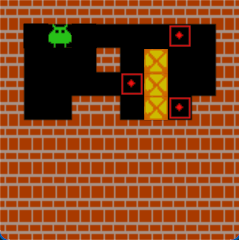
\includegraphics[width=1\textwidth]{Images/sokoban_cas_2.png}
\caption{\label{Graph.jpg} A graph showing the boundary of the relationship between the axion mass and axion coupling.}
\end{figure}

The left hand side of the graph (the flat line) is a graphical representation of the fact that, if the mass is very small, the coupling becomes independent of the mass of the axion. The right hand side of the graph shows that, if the mass is significantly large, the limit becomes dependent on a decaying trigonometric function. These results match up with figure 4 from the 'New ALPS results...' paper. This line does not, however, represent the only values that the mass and coupling can take,  as we recall that the probability of conversion used is the \textit{maximum} probability. Therefore, this line only represents a boundary between possible and im possible combinations of axion mass and coupling values, and rules out any combinations of values that lie above the line. Also notice that, for a low mass, figure 2 reads a coupling strength of $\approx 2\times 10^{-8} GeV^{-1} $, whereas, in figure 4 of the ALPS paper previously mentioned, the low mass coupling strength reads to be $\approx 5\times 10^{-7}GeV{-1}$. We see, in figure 2 that the large mass approximation starts to have effect at around $10^{-12} GeV$, which matches up very closely with figure 4 of the ALPS paper.

\section{Discussion}
\label{sec:discussion}
The difference in the two values for the low mass coupling strength may have been caused by a number of factors. Firsly, an assumption has been made, that, because $g \propto 1/M$, $g = 1/M$. No account has been made of a possible constant factor in the case where $g$ and $M$ are not directly inversely proportional.
Another error may have arisen due to the fact that we assumed that the quoted probability, $2.25 \times 10^{-25}$, was the probability that a photon $\rightarrow$ axion $\rightarrow$ photon conversion would take place, where it may have actually been that a single photon $\rightarrow$ axion / axion $\rightarrow$ photon conversion would occur. 
Some small errors may have also been introduced when converting constants, such as the magnetic field or the frequency of light, into electron volts to be in natural units. The constants, in natural units, were inputted to only 4 decimal places. To improve the accuracy of the values on the graph plotted in figure 2, these constants could be used to many more decimal places, especially when using an accurate program, such as MatLab. 
We must however take figure 2 with a pinch of salt, as there is obviously a large transition step between the small mass and large mass approximations. The closer the values are to the transition between the two approximations, the more unreliable the values are, as the original fraction we were using to approximate in equation $(17)$ becomes less dependent on just a single term of the denominator. 
Another assumption that has been made is that the refractive index inside the argon gas is equal to that of a vacuum, $n=1$, whereas the real refractive index is slightly higher than this. 

\section{Conclusions}
\label{sec:conclusions}

In this experiment, we have theoretically reproduced limits set on the mass and coupling strength of possible axionic particles, by using a series of mathematical calculations and physical and mathematical approximations. Our methods and approximations have arrived at a graph which qualitatively matches the most stringent constraints on the existence of axions. \\
In the future, the ALPS collaboration will continue with their research into the properties of axions and other weakly interacting particles, by increasing magnet strength and laser power, to increase the chances of photon $\rightarrow$ axion conversion. 

\printbibliography

\end{document}